\newcommand{\indepbm}{\psi}
\newcommand{\toinP}{\overset{\P}\to}
\newcommand{\statementoflemresampledetosampled}{$\resamplede \toinP \sampled$ as $\epsilon \to 0$}

\newcommand{\statewebO}{S_{\webnoargs}}
\newcommand{\statenowebO}{S_{\indepbm}}
\newcommand{\trajs}{\mathcal{X}}
\newcommand{\tensorcondition}{$\sigma$-fields $\F_a$, $\F_b$, $\F_c$
  we write $\F_a = \F_b \tensor \F_c$ when $\F_a$ is generated by
  $\F_b$ and $\F_c$ (up to sets of measure $0$), and $\F_b$ and $\F_c$
  are independent}
{
\section{Recovering the web from half-planes}
\label{sec:recovering-from-half-planes}

In this section we introduce three \sigfield{}s generated by the
Brownian web and use
them to restate Theorem \ref{thm:informal-recovering-from-half-planes}
as Theorem \ref{thm:recoveringfromhalfplanes}.

\newcommand{\restrictupper}{\mathcal{R}_{+}}

  Write $\trajs$ for the collection of trajectories comprising the whole web,
  that is $\{t \mapsto \web{s}{t}{x} : (s,x) \in \R^2\}$,
  and $\wholefield$ for the $\sigma$-field generated by the
  whole web, i.e.\ generated by $\trajs$.
  We further introduce $\upperhp$ and $\lowerhp$, the \sigfield{}s
  generated by the web on the upper and lower half-planes
  respectively.  Formally,

  \begin{definition*}
  For any path $f$ we write $\restrictupper(f)$ for $f$ stopped at the
  first time it is outside the upper half-plane.
  $\restrictupper(t \mapsto \web{s}{t}{x})$ is therefore the trajectory of the
  web $\webnoargs$ started at the point $(s,x)$ and stopped at the first
  time it is outside the upper half-plane (if $(s,x)$ is outside the
  upper half-plane, $f$ is stopped immediately).
  We define $\upperhp$ to be the $\sigma$-field generated by the
  collection of paths $\{\restrictupper(X) : X \in \trajs \}$, and define $\lowerhp$ analogously.
  \end{definition*}

  Note that $\upperhp$ and $\lowerhp$ are independent by the definition of
  a system of $n$ independent-coalescing Brownian motions.

  \newcommand{\F}{\mathcal{F}}
  For \tensorcondition{}.
  We are now ready to restate Theorem
  \ref{thm:informal-recovering-from-half-planes}.

\begin{theorem}\label{thm:recoveringfromhalfplanes}
  $\wholefield = \twostrips$.
\end{theorem}

The difficulty is to show that $\wholefield \subseteq \twostrips$,
because the reverse inclusion follows directly from the definitions.
To avoid having to state results as ``for all $\sampled \in \trajs$
\ldots'', here and for the rest of the paper we write $\sampled$ for
an arbitrary element of $\trajs$.  This we do purely for the sake of
notational simplicity.

$\wholefield$ is generated by such processes, so
using the third property in Definition~\ref{def:web}
our theorem reduces to the following lemma.

\begin{lemma}
  \label{lem:sampled-twostrip-meas}
  $\sampled$ is $\twostrips$-measurable.
\end{lemma}

To prove this we must show that $\sampled$ can be recovered using
trajectories starting in the upper half-plane which stop when they hit
$0$, and trajectories starting on the lower half-plane which stop when
they hit $0$.

To do so, we might have liked to recover $X$ (starting on, say, the
upper half-plane) by following it until it hits 0, then by following its
continuation within the lower half-plane.  However, this is impossible
since when trajectories of Brownian motion cross $0$ they do so
infinitely often within a finite period of time.

To overcome this problem we introduce in Section
\ref{subsec:the-perturbed-process} a process $\resamplede$, for each
$\epsilon > 0$, which is $\twostrips$-measurable.  In Section
\ref{sec:proof-of-lem:resamplede-to-sampled} we show that
$\resamplede$ is an approximation of $\sampled$ in the sense that
$\resamplede$ converges to $\sampled$ (in probability) as $\epsilon \to 0$.  This will
imply that $\sampled$ itself is $\twostrips$-measurable.

\subsection{The perturbed process}
\label{subsec:the-perturbed-process}

\TODO{}{Should we call this the approximation process?}

{
\newcommand{\joinernoargs}{\psi}
\newcommand{\joiner}[2]{\joinernoargs_{{#1}{#2}}}
\newcommand{\joinerval}[1]{\joinernoargs_{#1}}
  From our arbitrary $\sampled$ we now construct $\resamplede$, a
  ``perturbed'' version of $\sampled$, which depends also on
  $\joinerval{t}$,
  some Brownian motion independent of $\webnoargs$ (measurable with
  respect to $\reservoir$, say, where $\reservoir$ is independent of
  $\wholefield$).

  In the definition of $\resamplede$
  we give the word ``follows'' two distinct meanings.
  We say $\resamplede$ follows $\webnoargs$ on $[s,u]$ if
  $\resamplede_t = \web{s}{t}{\resamplede_s}$ for $t \in [s,u]$.
  That is if the trajectory of $\resamplede$ follows the trajectory of
  the web starting from point $\resamplede_s$ at time $s$ and up to time $u$.
  We say $\resamplede$ follows $\joinernoargs$ on $[s,u]$ if
  $\resamplede_t = \resamplede_s + \joinerval{t} - \joinerval{s}$ for $t \in [s,u]$.

\begin{definition}
  \label{def:resamplede}
  The perturbed process $\resamplede$ starts at the same time and position
  as $\sampled$ and
  alternates between two states.
  In state $\statewebO$ it follows
  $\webnoargs$ while, in state $\statenowebO$ it follows $\indepbm$.
  The process starts in state $\statewebO$ and
  the transition from state $\statewebO$ to state $\statenowebO$ occurs
  when $\resamplede$ hits $0$, while
  the transition from state $\statenowebO$ to state $\statewebO$ occurs when
  $\resamplede$ hits $\pm \epsilon$.
  \TODO{}{State why this definition is well-defined?}
  See Figure \ref{fig:perturbed} for an illustration of sample paths of
  $\sampled$ and $\resamplede$.
\end{definition}
}

\begin{figure}
   \centering%
   $\begin{array}{cc}
   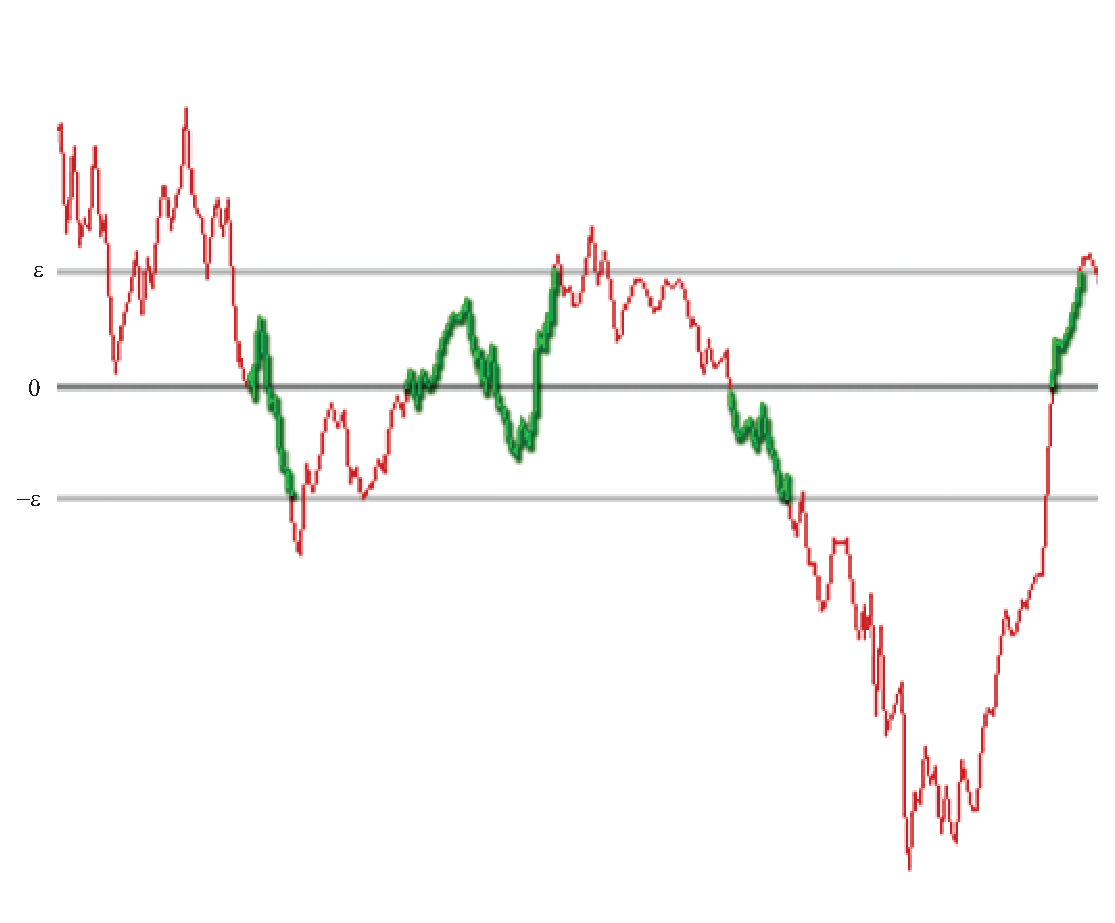
\includegraphics[scale=0.33]{resample1.eps}&
   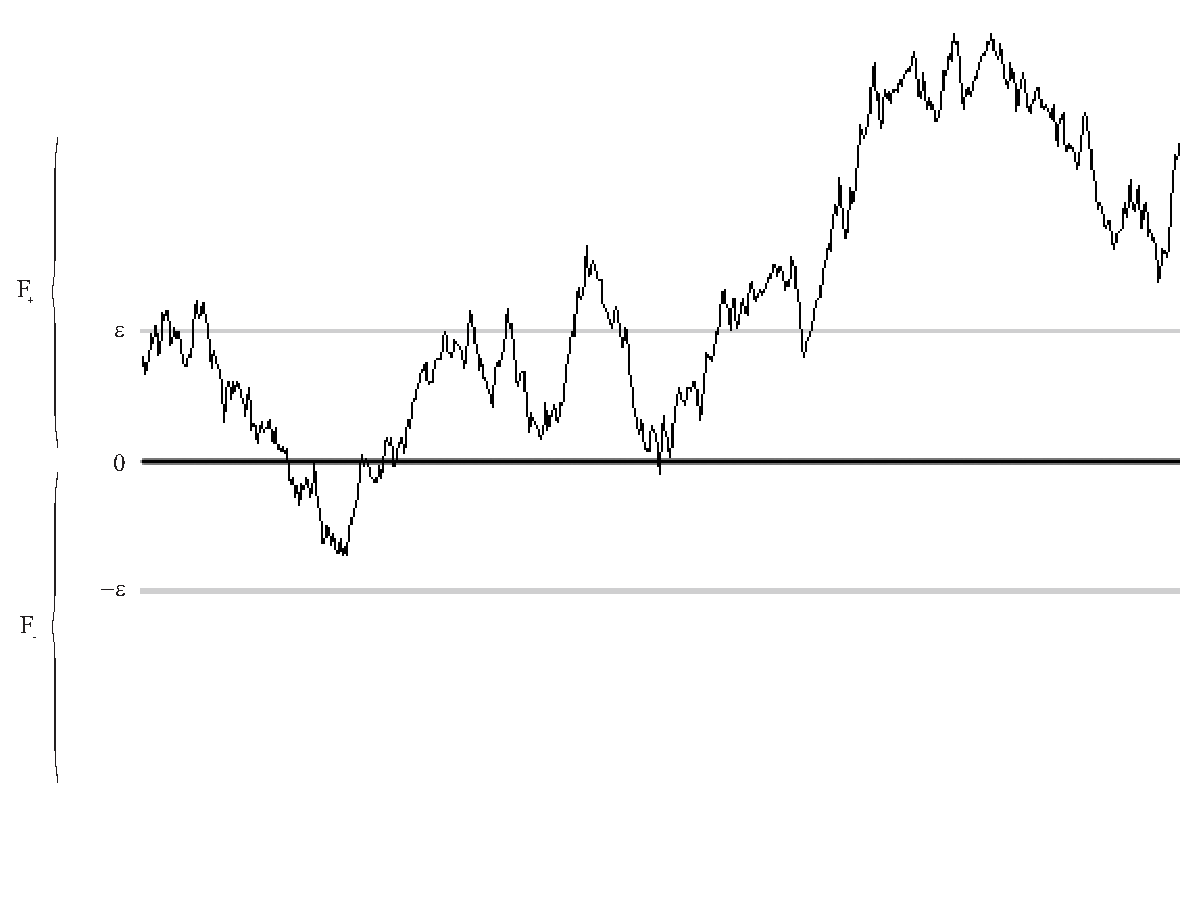
\includegraphics[scale=0.33]{resample2.eps}\\
   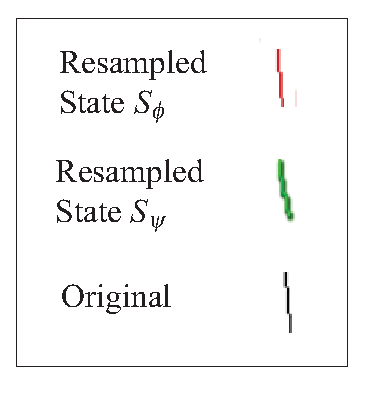
\includegraphics[scale=0.66]{state-glos.eps}&
   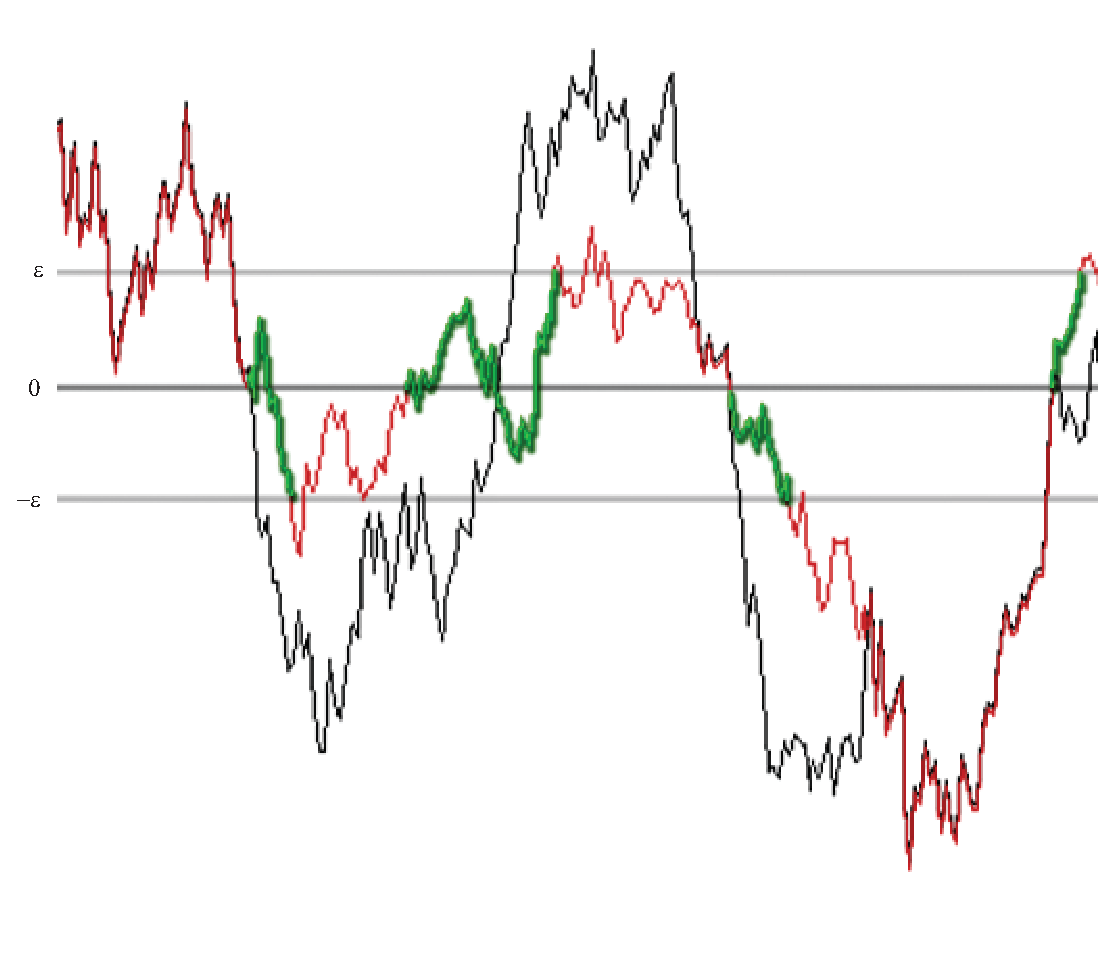
\includegraphics[scale=0.33]{resample.eps}
   \end{array}$
   \caption{
     \label{fig:perturbed}
   A sample of a web trajectory and the corresponding perturbed processes.
   The top left image depicts the perturbed process, with state $\statenowebO$ in bold.
   The top right image depicts the original web trajectory. The center image
   illustrates both processes together, showing the segments where they coalesce.
   }
\end{figure}

The following lemma specifies in what sense the perturbed process is
an approximation of the trajectory of the web.
Here and in the rest of the paper the convergence is uniform
on compacts in probability.

\begin{lemma}
  \label{lem:resamplede-to-sampled}
  \statementoflemresampledetosampled.
\end{lemma}
That is to say, for all $\delta > 0$, $u > s$
\[
\P(|\sampled(t) - \resamplede(t)| > \delta \text{ for some } t \in
  [s, u]) \to 0 \text{ as } \epsilon \to 0
\]
where $s$ is the time at which $\sampled$ and $\resamplede$ start.

Lemma \ref{lem:sampled-twostrip-meas} reduces to Lemma
\ref{lem:resamplede-to-sampled}.

\begin{proof}[Proof of reduction]
  $\resamplede$ is $\twostripsreservoir$-measurable, so we use Lemma
  \ref{lem:resamplede-to-sampled} to conclude that $\sampled$ is also
  $\twostripsreservoir$-measurable.  However, since $\sampled$ is
  actually independent of $\reservoir$ we can use a basic result on
  tensor products of Hilbert spaces (for example Equation (2c8) of
  \cite{tsirelson-noise-as-a-boolean-algebra}) to conclude that $\sampled$ is
  in fact $\twostrips$-measurable.
\end{proof}

We devote the following section to the proof of Lemma
\ref{lem:resamplede-to-sampled}.
}
